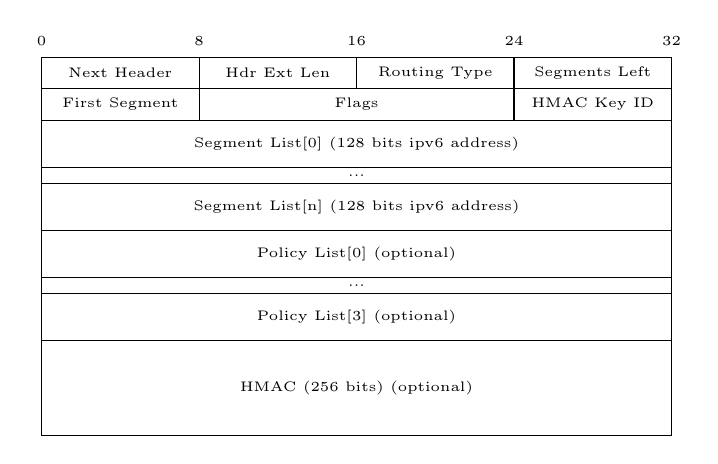
\begin{tikzpicture}[scale=2]%, show background rectangle]
	\node at (0, 2.5) {\tiny 0};
	\node at (1, 2.5) {\tiny 8};
	\node at (2, 2.5) {\tiny 16};
	\node at (3, 2.5) {\tiny 24};
	\node at (4, 2.5) {\tiny 32};

	\draw (0,2.2) rectangle (1,2.4) node[pos=.5] {\tiny Next Header};
	\draw (1,2.2) rectangle (2,2.4) node[pos=.5] {\tiny Hdr Ext Len};
	\draw (2,2.2) rectangle (3,2.4) node[pos=.5] {\tiny Routing Type};
	\draw (3,2.2) rectangle (4,2.4) node[pos=.5] {\tiny Segments Left};

	\draw (0,2.0) rectangle (1,2.2) node[pos=.5] {\tiny First Segment};
	\draw (1,2.0) rectangle (3,2.2) node[pos=.5] {\tiny Flags};
	\draw (3,2.0) rectangle (4,2.2) node[pos=.5] {\tiny HMAC Key ID};

	\draw (0,1.7) rectangle (4,2.0) node[pos=.5] {\tiny Segment List[0] (128 bits ipv6 address)};
	\draw (0,1.6) rectangle (4,1.7) node[pos=.5] {\tiny ...};
	\draw (0,1.3) rectangle (4,1.6) node[pos=.5] {\tiny Segment List[n] (128 bits ipv6 address)};
	\draw (0,1.0) rectangle (4,1.3) node[pos=.5] {\tiny Policy List[0] (optional)};
	\draw (0,0.9) rectangle (4,1.0) node[pos=.5] {\tiny ...};
	\draw (0,0.6) rectangle (4,0.9) node[pos=.5] {\tiny Policy List[3] (optional)};
	\draw (0,0.0) rectangle (4,0.6) node[pos=.5] {\tiny HMAC (256 bits) (optional)};
\end{tikzpicture}
